\appendix
\section{Anhang}
\label{sec:appendix}

\begin{lstlisting}[caption=Abstract file storage strategy, label=code:strategyinterface]
class AbstractFileStorageStrategy {
	constructor() {
		if (new.target === AbstractFileStorageStrategy) {
			throw new TypeError("Cannot construct AbstractFileStorageStrategy instances directly.");
		}
	}
	
	create() {
		throw new TypeError("create method has to be implemented.");
	}
	
	getFiles() {
		throw new TypeError("getFiles method has to be implemented.");
	}
	
	deleteFile() {
		throw new TypeError("deleteFile method has to be implemented.");
	}
	
	generateSignedUrl() {
		throw new TypeError("generateSignedUrl method has to be implemented.");
	}
	
	createDirectory() {
		throw new TypeError("createDirectory method has to be implemented.");
	}
	
	deleteDirectory() {
		throw new TypeError("deleteDirectory method has to be implemented.");
	}
}

module.exports = AbstractFileStorageStrategy;
\end{lstlisting}

\begin{lstlisting}[caption=Registrieren des FileStorage Services, label=code:filestorageindex]
	module.exports = function () {
		const app = this;
		
		// Registriert die drei Services
		app.use('/fileStorage/directories', new DirectoryService());
		app.use('/fileStorage/signedUrl', new SignedUrlService());
		app.use('/fileStorage', new FileStorageService());
		
		// Holt die registrierten Services, um die Hooks zu initialisieren
		const fileStorageService = app.service('/fileStorage');
		const signedUrlService = app.service('/fileStorage/signedUrl');
		const directoryService = app.service('/fileStorage/directories');
		
		// Initialisiere "Before"-Hooks
		fileStorageService.before(hooks.before);
		signedUrlService.before(hooks.before);
		directoryService.before(hooks.before);
		
		// Initialisiere "After"-Hooks
		fileStorageService.after(hooks.after);
		signedUrlService.after(hooks.after);
		directoryService.after(hooks.after);
	};
\end{lstlisting}


\begin{lstlisting}[caption=deleteFile() Funktion der AWS S3-Strategy, label=code:awsS3deletefile]
	deleteFile(userId, path) {
		if (!userId || !path) return Promise.reject(new errors.BadRequest('Missing parameters'));
	
		// prüfe Berechtigung für die Löschen-Aktion
		return filePermissionHelper.checkPermissions(userId, path, ['can-write'])
	
			// finde gegeben Nutzer in Datenbank
			.then(res => UserModel.findById(userId).exec())
				.then(result => {
					if (!result || !result.schoolId) return Promise.reject(errors.NotFound("User not found"));
		
					// erstelle AWS-Verbindungsobjekts
					const awsObject = createAWSObject(result.schoolId);
		
					// stelle Parameter für das Löschen der Datei ein
					const params = {
						Bucket: awsObject.bucket,
						Delete: {
							Objects: [
								{
									Key: path
								}
							],
							Quiet: true
						}
					};
		
					// Führe Aktion aus
					return promisify(awsObject.s3.deleteObjects, awsObject.s3)(params);
		});
	}
\end{lstlisting}

\begin{lstlisting}[caption=checkNormalPermissions() Funktion des filePermissionHelper, label=code:fphnormal]
	checkNormalPermissions(userId, filePath) {
		let values = filePath.split("/");
		if (values[0] === '') values = values.slice(1);
		if (values.length < 2) return Promise.reject(new errors.BadRequest("Path is invalid"));
		const contextType = values[0];
		const contextId = values[1];
		switch (contextType) {
			case 'users':
			
				// überprüfe, ob zu Prüfender Besitzer der Datei ist
				if (contextId !== userId.toString()) {
					return Promise.reject(new errors.Forbidden("You don't have permissions!"));
				} else {
					return Promise.resolve();
				}
				
			case 'courses':
			
			// überprüfe, a) ob der Nutzer zum Kurs gehört, b) ob der Kurs überhaupt existiert
			return CourseModel.find({
				$and: [
					{$or: [{userIds: userId}, {teacherIds: userId}]},
					{_id: contextId}
				]
			}).exec().then(res => {
				if (!res || res.length <= 0) {
					return Promise.reject(new errors.Forbidden("You don't have permissions!"));
				}
				
				return Promise.resolve(res);
			});
			
		case 'classes':
			
			// überprüfe, a) ob der Nutzer zur Klasse gehört, b) ob die Klasse überhaupt existiert
			return ClassModel.find({
				$and: [
					{$or: [{userIds: userId}, {teacherIds: userId}]},
					{_id: contextId}
				]
			}).exec().then(res => {
				if (!res || res.length <= 0) {
					return Promise.reject(new errors.Forbidden("You don't have permissions!"));
				}
			
			return Promise.resolve(res);
		});
		
		default:
			return Promise.reject(new errors.BadRequest("Path is invalid"));
		}
	}
\end{lstlisting}

\begin{lstlisting}[caption=checkExtraPermissions() Funktion des filePermissionHelper, label=code:fphextra]
	checkExtraPermissions(userId, fileKey, permissionTypes) {
		if (!fileKey || fileKey === '') return Promise.reject(new errors.Forbidden("You don't have permissions!"));
	
		return FilePermissionModel.find({key: fileKey}).exec().then(res => {
		
		// Datenbankobjekt sollte einzigartig für Datei sein, trotzdem werden mehrere Einträge hier zusammengefasst
		let permissions = _.flatten(res.map(filePermissions => filePermissions.permissions));
	
		// versuche Datenbankeintrag für bestimmten Nutzer zu finden
		let permissionExists = permissions.filter(p => {
			return JSON.stringify(userId) === JSON.stringify(p.userId) && _.difference(permissionTypes, p.permissions).length === 0;
		}).length > 0;
	
		if (!permissionExists) return Promise.reject(new errors.Forbidden("You don't have permissions!"));
	
		return Promise.resolve();
		}).catch(err => {
			return Promise.reject(new errors.Forbidden("You don't have permissions!"));
		});
	}
\end{lstlisting}

\begin{figure}[H]
	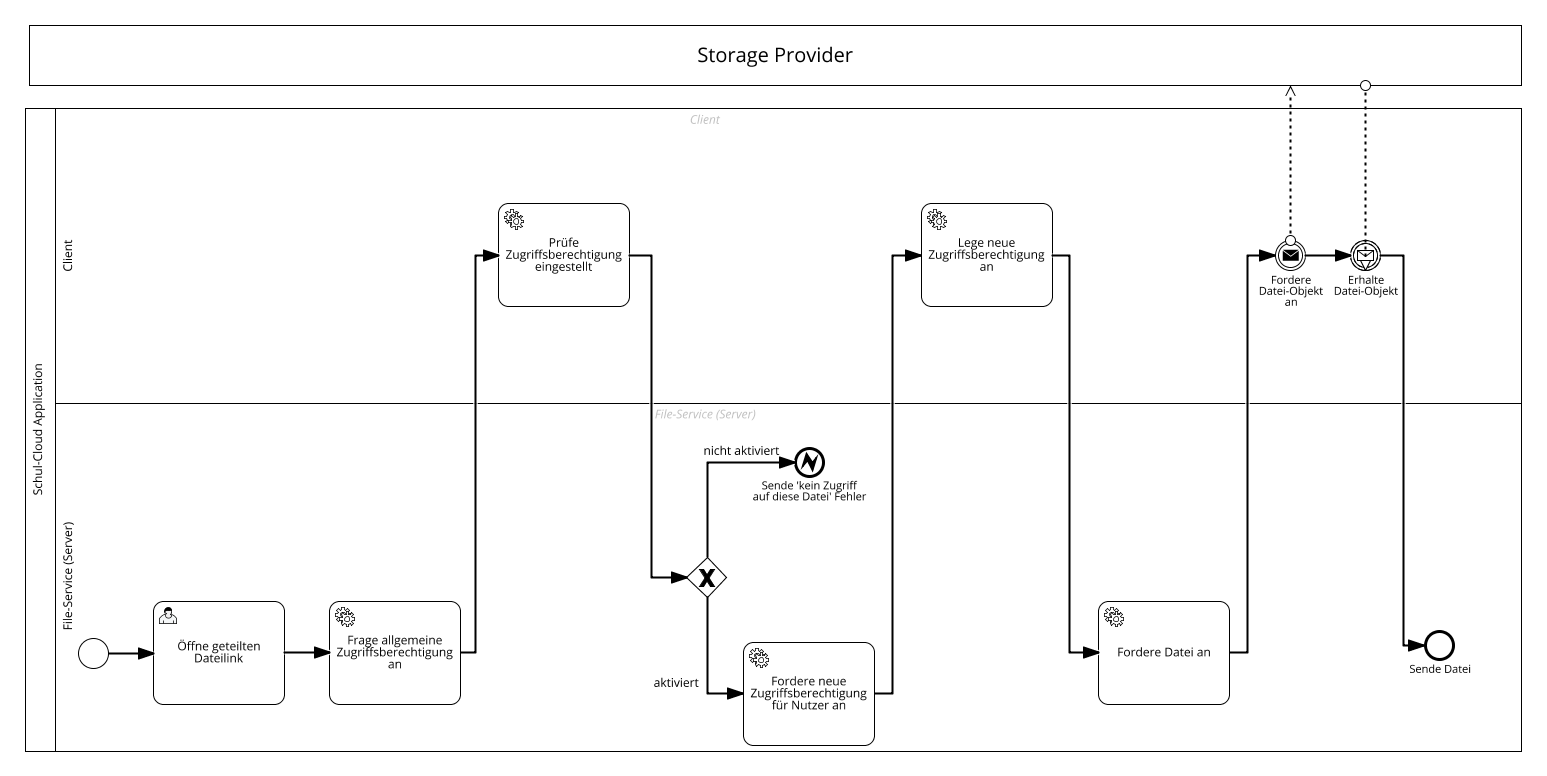
\includegraphics[width=1.5\linewidth, angle=270]{images/filesharingusing}
	\caption[Caption for concept]{Zugriff auf eine geteilte Datei}
	\centering
	\label{fig:filesharingusing}
\end{figure}

\begin{figure}[H]
	\centering
	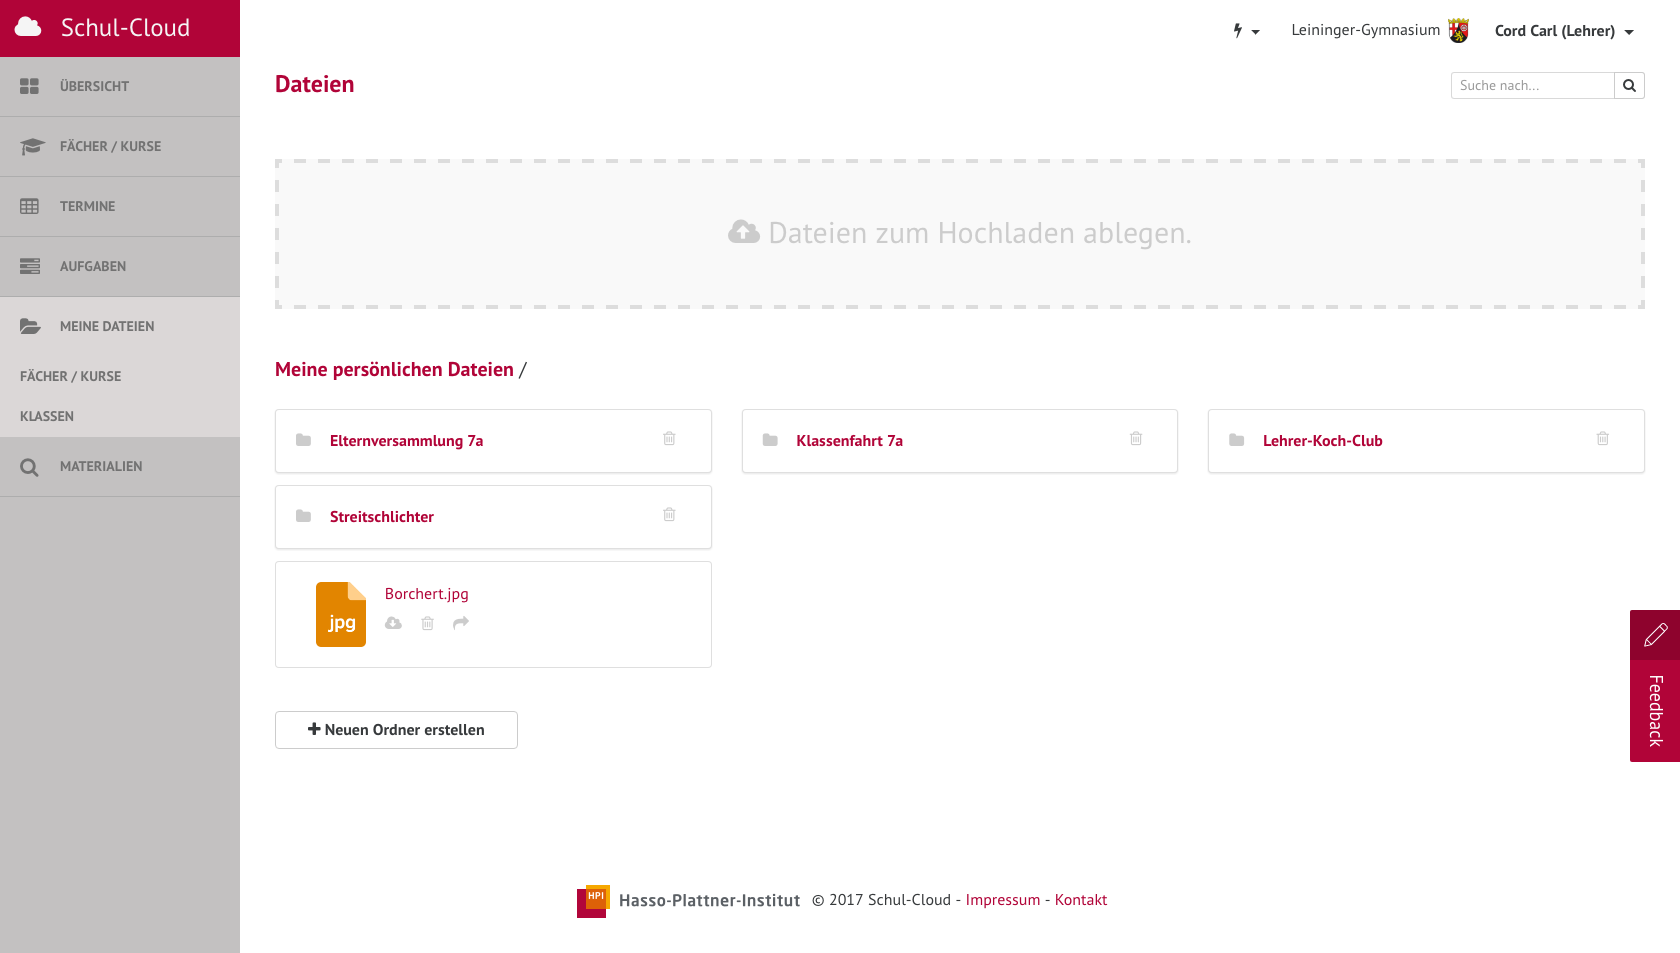
\includegraphics[width=1\linewidth]{images/screenMeineDateien}
	\caption{Ansicht für die persönlichen Dateien}
	\label{fig:screenMeineDateien}
\end{figure}

\begin{figure}[H]
	\centering
	\includegraphics[width=1\linewidth]{images/screenCkEditor}
	\caption{Ansicht für das Hinzufügen einer Datei in den Unterrichtskontext}
	\label{fig:screenCkEditor}
\end{figure}

\begin{figure}[H]
	\centering
	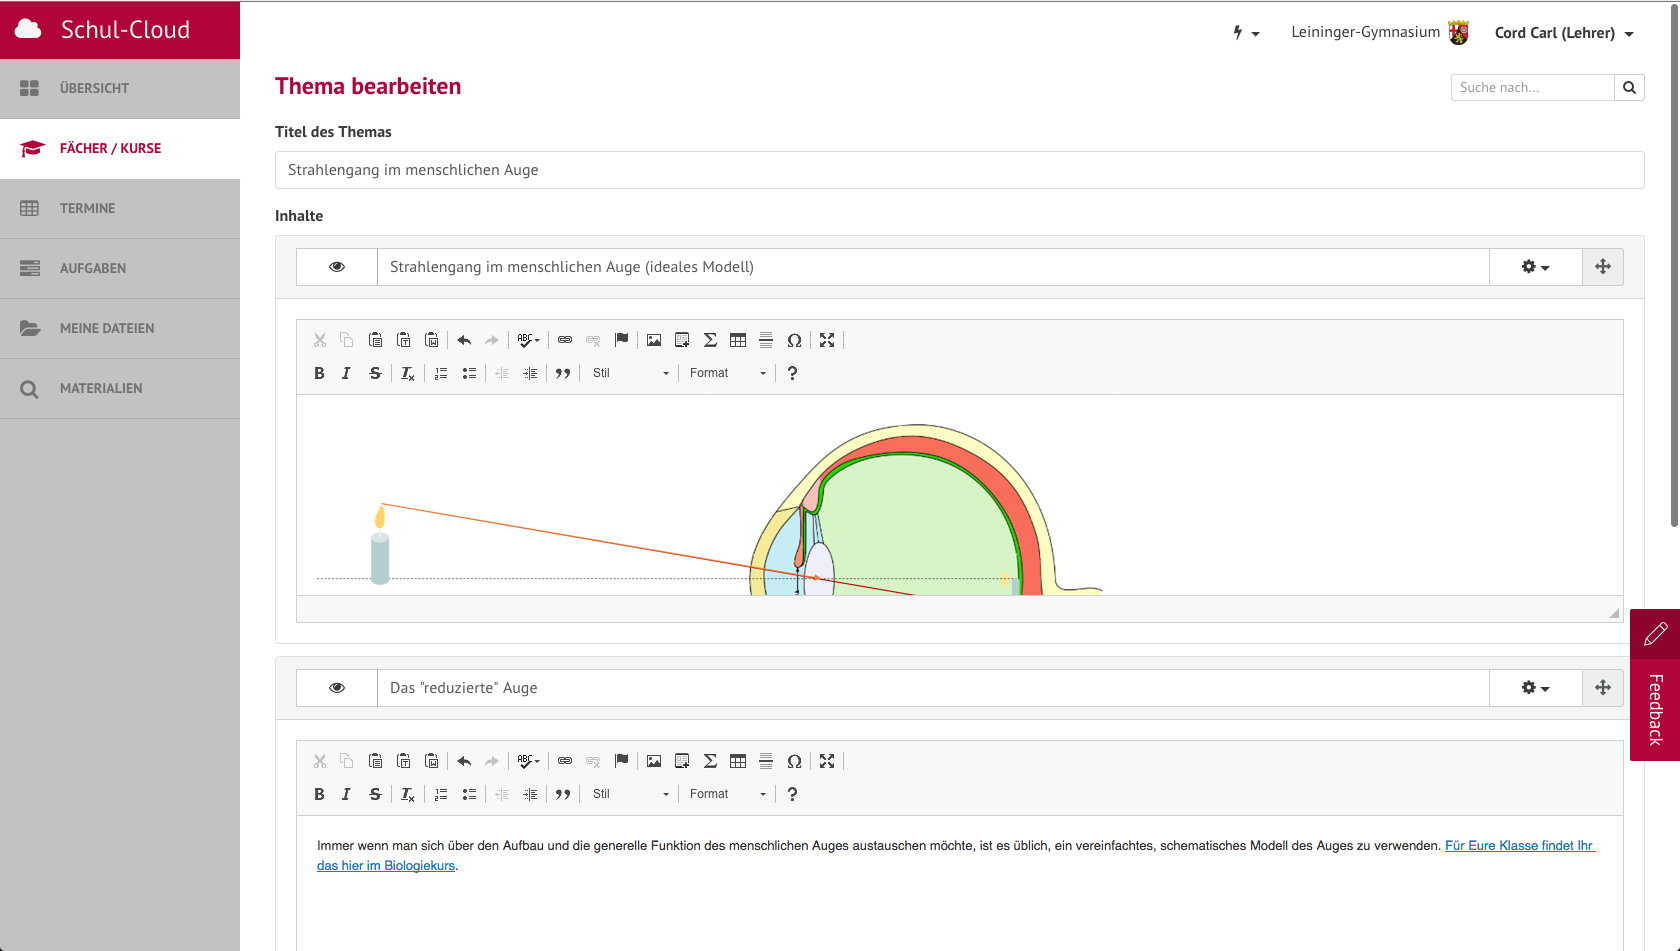
\includegraphics[width=1\linewidth]{images/editor_picture}
	\caption{Ansicht einer Datei als Lernelement im Themeneditor}
	\label{fig:screenTopicEditor}
\end{figure}

\begin{figure}[H]
	\centering
	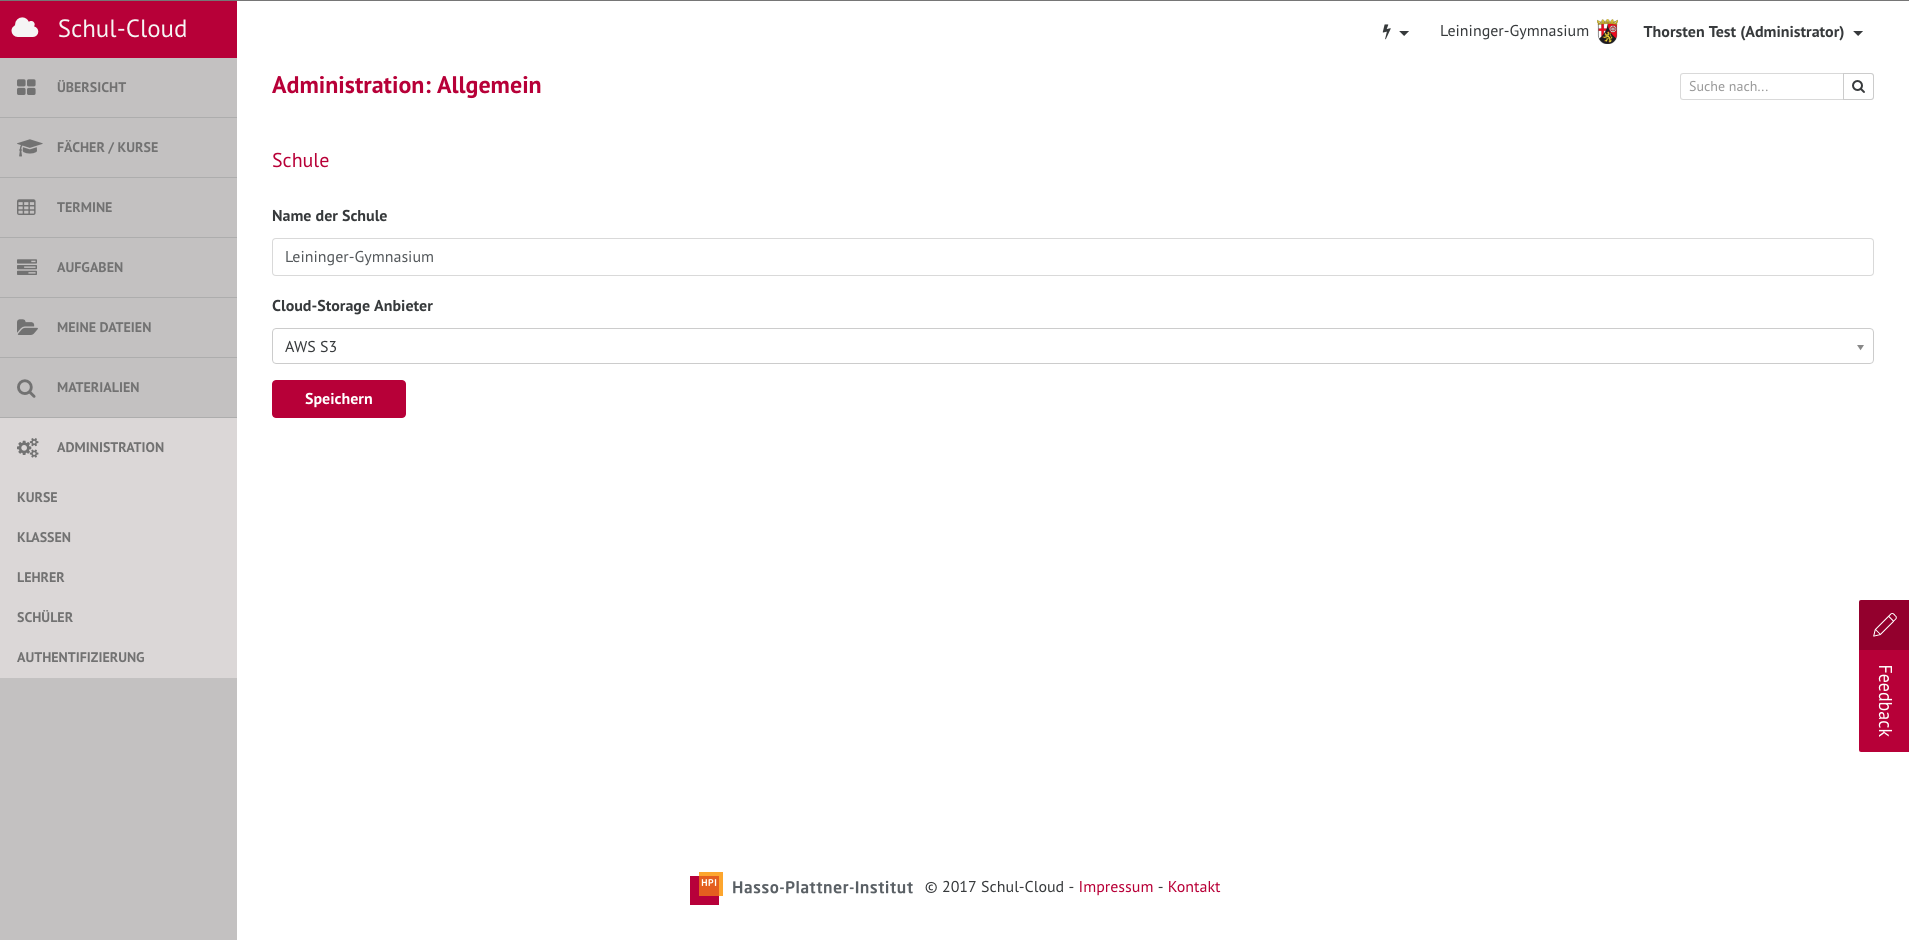
\includegraphics[width=1\linewidth]{images/adminFileStorage}
	\caption{Ansicht für die Auswahl des File Storage Providers}
	\label{fig:adminFileStorage}
\end{figure}

\begin{figure}[H]
	\centering
	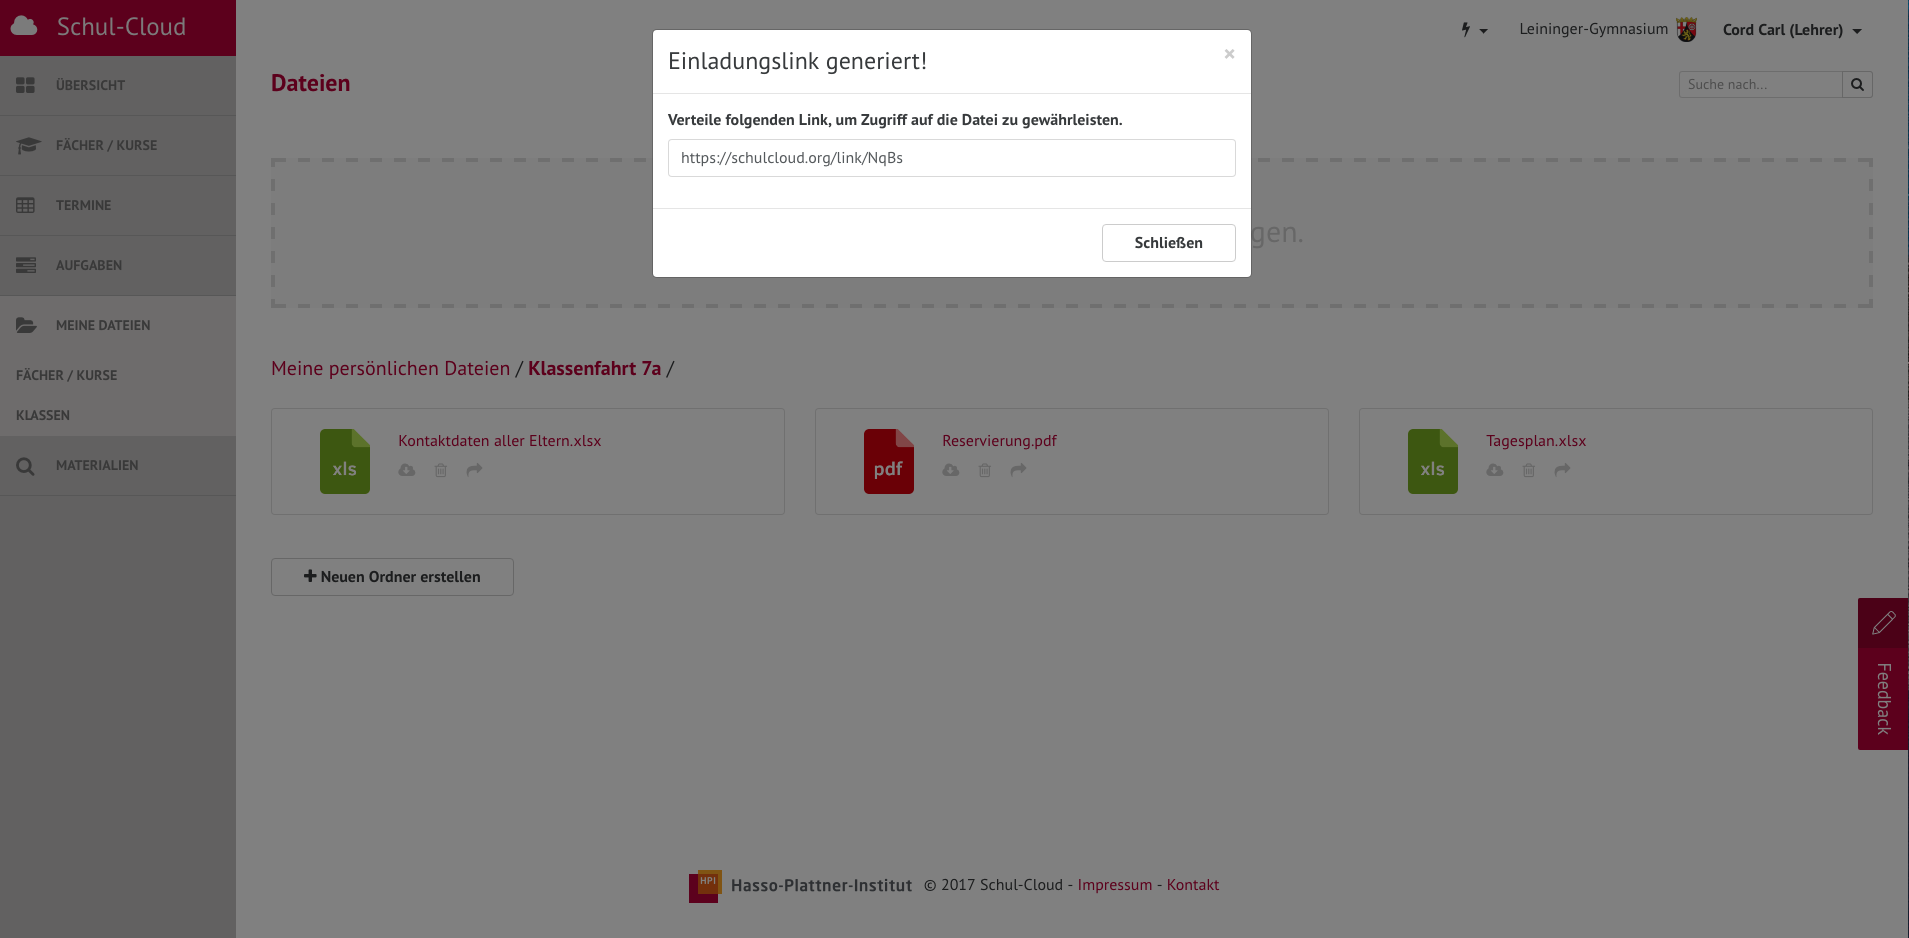
\includegraphics[width=1\linewidth]{images/sharingfileui}
	\caption{Ansicht für das Erstellen eines Zugriffslinks}
	\label{fig:sharingfileui}
\end{figure}
\clearpage